\question
(0,5 балла) Попав в незнакомый город на один день, вы и двое ваших друзей решили пройти по всем интересным вам местам. Условная карта города приведена ниже.

\begin{minipage}[h]{0.45\linewidth}
\center{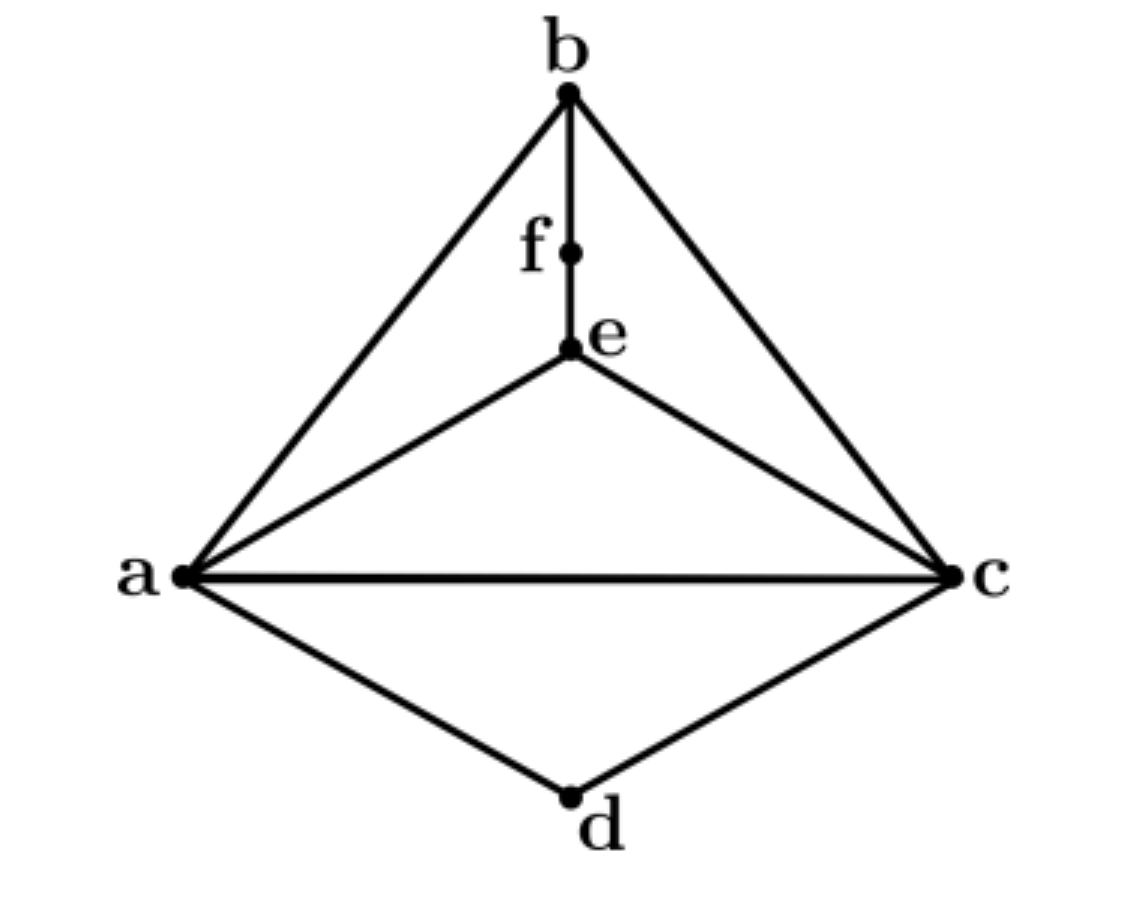
\includegraphics[width=0.7\textwidth]{pic/35.png} }
\end{minipage}

Проблема в том, что вы никак не можете договориться о маршруте. Чтобы прийти к компромиссу, надо найти следующие параметры графа города:
\begin{itemize}
\item три разных остовных дерева (то есть маршруты каждого из вашей компании)
\item центр
\item диаметр
\item радиус
\end{itemize}

Также надо понять, какие маршруты можно составить, если вы успеете не всё:
\begin{itemize}
\item цепь длины 6
\item замкнутый путь длины 10
\item вершинно-простой путь длины 5
\item цикл длины 4 и 6
\item простой цикл длины 3 и 4
\end{itemize}
